\documentclass[a4paper, 11pt]{article}

\setcounter{tocdepth}{3}
\setcounter{secnumdepth}{3}

\usepackage{comment} % enables the use of multi-line comments (\ifx \fi) 
\usepackage{lipsum} %This package just generates Lorem Ipsum filler text. 
\usepackage{fullpage} % changes the margin
\usepackage[utf8]{inputenc}
\usepackage{gensymb}
\usepackage{graphicx}
\usepackage{booktabs}% http://ctan.org/pkg/booktabs
\usepackage{makecell}
\usepackage{tabularx}
\usepackage[table]{xcolor}
\usepackage{array}
\usepackage{wrapfig}
\usepackage{subcaption}
\usepackage{csquotes}
\usepackage{lscape}
\usepackage{afterpage}
\usepackage{geometry}
\usepackage{listings}
\usepackage{chngcntr}
\usepackage{multicol}

\counterwithin{figure}{section}

\geometry{a4paper, margin=1in}
\renewcommand{\figurename}{Abb.}
\renewcommand{\tablename}{Tabelle}
\newcommand{\code}[1]{\texttt{#1}}

\renewcommand*{\thead}[1]{\bfseries #1}

\renewcommand{\contentsname}{Inhalt}
\renewcommand{\listfigurename}{Abbildungsverzeichnis}


\begin{document}
 
\title{Einführung in die Internationalen Beziehungen - HS2018}
\author{Alex Neher}
\maketitle

\tableofcontents
\newpage
\listoffigures
\newpage

\graphicspath{{./Pictures/}}


\section{Einführung}
\subsection{Definitionen}
\subsubsection{Politikwissenschaft}
Die Definition der Politikwissenschaften hat sich mit der Zeit verändert:
\begin{description}
    \item[Traditionell:] Handlungen des Staates und seiner Organe verstehen
    \item[Modern:] Breites Verständnis des Politischen aneignen
    \item[Heute:] Das Zusammenspiel zwischen Staat und Gesellschaft verstehen
\end{description}        

\vspace{10px}
\noindent Die heutige Politiwissenschaft lässt sich in verschiedene Subkategorien unterteilen:
\begin{multicols}{2}
    \begin{itemize}
        \item Das Politische System
        \item Vergleichende Politikwissenschaften
        \item Internationale Beziehungen
\columnbreak
        \item Politische Theorie
        \item Methodenlehre
        \item Politisches Verhalten
    \end{itemize}
\end{multicols}

\subsubsection{Politik}
Der Begriff 'Politik' ist folgendermassen definiert:

\begin{center}
    \blockquote{Soziales Handeln, das auf Entscheidungen und Steuerungsmechanismen ausgerichtet ist, die allgemein verbindlich sind und das Zusammenleben von Menschen regeln.}
\end{center}

Die Politik lässt sich grundsätzlich in drei Arten unterteilen. In der Deutschen Sprache werden für alle drei Begriffe dasselbe Wort verwendet, im Englischen kann jedoch unterschieden werden zwischen: 
\begin{description}
    \item[Policy: ] \textit{Was} - Inhalte der Politik. Regeln, Weisungen
    \item[Polity:] \textit{Wer} - Die Strukturen und Akteure der Politik.  Organisationen, Parteien 
    \item[Politics:]  \textit{Wie} - Die Prozesse, wie Regeln, Weisungen etc. entstehen.
\end{description}

\subsubsection{Staat}
Ein Staat benötigt laut dem Völkerrecht mind. die folgenden drei Elemente, um als Staat anerkannt zu werden: 
\begin{description}
    \item[Staatsgebiet: ] Ein Gebiet, über welches der Staat die alleinige Macht hat
    \item[Staatsvolk: ] Ein Volk, welches im Staatsgebiet lebt und unter der Staatsgewalt des Staates ist.
    \item[Staatsgewalt: ] Der Staat hat das Recht, Gesetze zu erlassen und diese durchzusetzen. Er darf Steuern erlassen, um öffentliche Güter bereitzustellen oder Einkommen umzuverteilen. Jedoch muss der Staat die innere und äussere Sicherheit garantieren können.
\end{description}

\begin{figure}[htb]
    \centering
    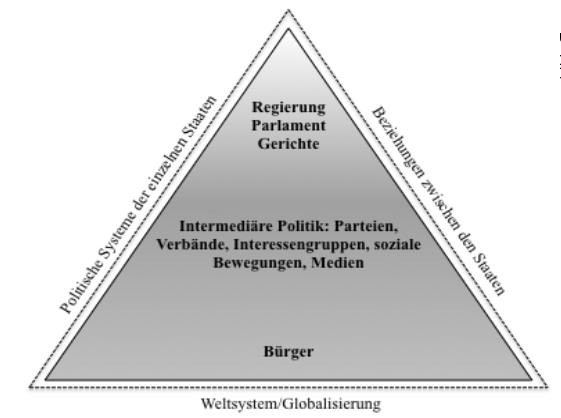
\includegraphics[keepaspectratio=true,height=15\baselineskip]{analytische_grundstruktur.png}
    \caption{Grundstruktur eines Staates}
    \label{fig:grundstrk_staat}
\end{figure}

Die Interessen der Staatsbürger werden meist über sogenannte \textit{Intermediärorgane} gewahrt. Das sind z.B. Parteien, Organisationan o.ä; Kurz gesagt, Polity.

\newpage

\subsection{Internationale Beziehungen}

Durch das Studium von internationalen Beziehungen versucht man zu verstehen, wie verschiedene Völker miteinander umgehen und miteinander auskommen. Die untersuchten Beziehungen können sowohl von freundschaftlicher, wie aber auch von kriegerischer Natur sein.

\vspace{10px}

Schimmelfennig beschreibt die internationale Politik als \blockquote[Schimmelfennig 2015, p.19]{Gesamtheit aller Interaktionen, die auf die autoritative Verteilung von Werten jenseits staatlicher Grenzen gerichtet sind}. Soll heissen; Alle Bemühungen, eine internationale Gesellschaft aufzubauen, die nach ähnlichen oder den gleichen Werten strebt.

\vspace{10px}

Im Gegensatz zur nationalen Politik, in welcher es eine Regierung in irgendeiner Form (Parlament, König o.ä) gibt, herrscht in der internationalen Politik \textbf{Anarchie}. Es gibt \textbf{keine zentrale Autorität} im internationalen System. Jegliche Allianzen und Kooperationen die zwischen Staaten existieren sind selbstbestimmt. Sie bleiben nur solange bestehen, wie der stärkere der beiden Staaten einen Gewinn daraus ziehen kann.

Diese Anarchie im internationalen Umfeld stellt die einzelnen Staaten je nach dem vor schwer zu lösende Probleme. Prinzipiell sind es dieselben Probleme, die sie auch staatsintern zu meistern haben, jedoch herrscht dort keine Anarchie (oder sollte zumindest nicht)

Grundsätzlich lassen sich diese Probleme in drei Hauptkategorien unterteilen:

\begin{description}
    \item[Sicherheit: ] Der Staat hat für seine eigene Sicherheit zu sorgen. Im internationalen Umfeld gibt es kein Gewaltmonopol
    \end{description}        
\end{document}
